\mbox{$\displaystyle -\,$\,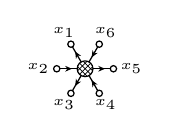
\begin{tikzpicture}[x=0.500cm, y=0.500cm, line width=0.450pt, baseline={([yshift=-0.6ex]0,0)}]
  \draw (0.000,0.000) -- (-0.360,0.624);
  \fill (-0.253,0.439) -- (-0.231,0.251) -- (-0.195,0.337) -- (-0.102,0.326) -- cycle;
  \draw (0.000,0.000) -- (-0.360,-0.624);
  \fill (-0.253,-0.439) -- (-0.102,-0.326) -- (-0.195,-0.337) -- (-0.231,-0.251) -- cycle;
  \draw (0.000,0.000) -- (0.720,0.000);
  \fill (0.507,0.000) -- (0.333,0.074) -- (0.390,0.000) -- (0.333,-0.074) -- cycle;
  \draw (-0.720,0.000) -- (0.000,0.000);
  \fill (-0.333,0.000) -- (-0.507,0.074) -- (-0.450,0.000) -- (-0.507,-0.074) -- cycle;
  \draw (0.360,-0.624) -- (0.000,0.000);
  \fill (0.167,-0.288) -- (0.189,-0.476) -- (0.225,-0.390) -- (0.318,-0.402) -- cycle;
  \draw (0.360,0.624) -- (0.000,0.000);
  \fill (0.167,0.288) -- (0.318,0.402) -- (0.225,0.390) -- (0.189,0.476) -- cycle;
  \fill[white] (0.000,0.000) circle (0.200);
  \draw[line width=0.248pt] (-0.193,-0.052) -- (0.052,0.193) (-0.141,-0.141) -- (0.141,0.141) (-0.052,-0.193) -- (0.193,0.052) (-0.193,0.052) -- (0.052,-0.193) (-0.141,0.141) -- (0.141,-0.141) (-0.052,0.193) -- (0.193,-0.052);
  \draw (0.000,0.000) circle (0.200);
  \draw[fill=white] (-0.360,0.624) circle (0.080);
  \draw[fill=white] (-0.720,0.000) circle (0.080);
  \draw[fill=white] (-0.360,-0.624) circle (0.080);
  \draw[fill=white] (0.360,-0.624) circle (0.080);
  \draw[fill=white] (0.720,0.000) circle (0.080);
  \draw[fill=white] (0.360,0.624) circle (0.080);
  \node[font=\tiny, inner sep=0pt, anchor=300] at (-0.445,0.771) {$x_{1}$};
  \node[font=\tiny, inner sep=0pt, anchor=0] at (-0.890,0.000) {$x_{2}$};
  \node[font=\tiny, inner sep=0pt, anchor=60] at (-0.445,-0.771) {$x_{3}$};
  \node[font=\tiny, inner sep=0pt, anchor=120] at (0.445,-0.771) {$x_{4}$};
  \node[font=\tiny, inner sep=0pt, anchor=180] at (0.890,0.000) {$x_{5}$};
  \node[font=\tiny, inner sep=0pt, anchor=240] at (0.445,0.771) {$x_{6}$};
\end{tikzpicture}}
\diagramgap
\mbox{$\displaystyle +\,$\,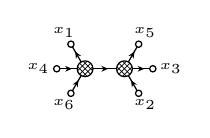
\begin{tikzpicture}[x=0.500cm, y=0.500cm, line width=0.450pt, baseline={([yshift=-0.6ex]0,0)}]
  \draw (-0.500,0.000) -- (-0.860,0.624);
  \fill (-0.753,0.439) -- (-0.731,0.251) -- (-0.695,0.337) -- (-0.602,0.326) -- cycle;
  \draw (0.500,0.000) -- (1.220,0.000);
  \fill (1.007,0.000) -- (0.833,0.074) -- (0.890,0.000) -- (0.833,-0.074) -- cycle;
  \draw (0.500,0.000) -- (0.860,0.624);
  \fill (0.753,0.439) -- (0.602,0.326) -- (0.695,0.337) -- (0.731,0.251) -- cycle;
  \draw (0.860,-0.624) -- (0.500,0.000);
  \fill (0.667,-0.288) -- (0.689,-0.476) -- (0.725,-0.390) -- (0.818,-0.402) -- cycle;
  \draw (-1.220,0.000) -- (-0.500,0.000);
  \fill (-0.833,0.000) -- (-1.007,0.074) -- (-0.950,0.000) -- (-1.007,-0.074) -- cycle;
  \draw (-0.860,-0.624) -- (-0.500,0.000);
  \fill (-0.667,-0.288) -- (-0.818,-0.402) -- (-0.725,-0.390) -- (-0.689,-0.476) -- cycle;
  \draw (-0.500,0.000) -- (0.500,0.000);
  \fill (0.087,0.000) -- (-0.087,0.074) -- (-0.030,0.000) -- (-0.087,-0.074) -- cycle;
  \fill[white] (-0.500,0.000) circle (0.200);
  \draw[line width=0.248pt] (-0.693,-0.052) -- (-0.448,0.193) (-0.641,-0.141) -- (-0.359,0.141) (-0.552,-0.193) -- (-0.307,0.052) (-0.693,0.052) -- (-0.448,-0.193) (-0.641,0.141) -- (-0.359,-0.141) (-0.552,0.193) -- (-0.307,-0.052);
  \draw (-0.500,0.000) circle (0.200);
  \fill[white] (0.500,0.000) circle (0.200);
  \draw[line width=0.248pt] (0.307,-0.052) -- (0.552,0.193) (0.359,-0.141) -- (0.641,0.141) (0.448,-0.193) -- (0.693,0.052) (0.307,0.052) -- (0.552,-0.193) (0.359,0.141) -- (0.641,-0.141) (0.448,0.193) -- (0.693,-0.052);
  \draw (0.500,0.000) circle (0.200);
  \draw[fill=white] (-0.860,0.624) circle (0.080);
  \draw[fill=white] (0.860,-0.624) circle (0.080);
  \draw[fill=white] (1.220,0.000) circle (0.080);
  \draw[fill=white] (-1.220,0.000) circle (0.080);
  \draw[fill=white] (0.860,0.624) circle (0.080);
  \draw[fill=white] (-0.860,-0.624) circle (0.080);
  \node[font=\tiny, inner sep=0pt, anchor=300] at (-0.945,0.771) {$x_{1}$};
  \node[font=\tiny, inner sep=0pt, anchor=120] at (0.945,-0.771) {$x_{2}$};
  \node[font=\tiny, inner sep=0pt, anchor=180] at (1.390,0.000) {$x_{3}$};
  \node[font=\tiny, inner sep=0pt, anchor=0] at (-1.390,0.000) {$x_{4}$};
  \node[font=\tiny, inner sep=0pt, anchor=240] at (0.945,0.771) {$x_{5}$};
  \node[font=\tiny, inner sep=0pt, anchor=60] at (-0.945,-0.771) {$x_{6}$};
\end{tikzpicture}}
\diagramgap
\mbox{$\displaystyle -\,$\,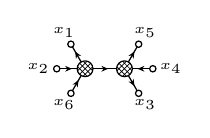
\begin{tikzpicture}[x=0.500cm, y=0.500cm, line width=0.450pt, baseline={([yshift=-0.6ex]0,0)}]
  \draw (-0.500,0.000) -- (-0.860,0.624);
  \fill (-0.753,0.439) -- (-0.731,0.251) -- (-0.695,0.337) -- (-0.602,0.326) -- cycle;
  \draw (0.500,0.000) -- (0.860,-0.624);
  \fill (0.753,-0.439) -- (0.731,-0.251) -- (0.695,-0.337) -- (0.602,-0.326) -- cycle;
  \draw (0.500,0.000) -- (0.860,0.624);
  \fill (0.753,0.439) -- (0.602,0.326) -- (0.695,0.337) -- (0.731,0.251) -- cycle;
  \draw (-1.220,0.000) -- (-0.500,0.000);
  \fill (-0.833,0.000) -- (-1.007,0.074) -- (-0.950,0.000) -- (-1.007,-0.074) -- cycle;
  \draw (1.220,0.000) -- (0.500,0.000);
  \fill (0.833,0.000) -- (1.007,-0.074) -- (0.950,0.000) -- (1.007,0.074) -- cycle;
  \draw (-0.860,-0.624) -- (-0.500,0.000);
  \fill (-0.667,-0.288) -- (-0.818,-0.402) -- (-0.725,-0.390) -- (-0.689,-0.476) -- cycle;
  \draw (-0.500,0.000) -- (0.500,0.000);
  \fill (0.087,0.000) -- (-0.087,0.074) -- (-0.030,0.000) -- (-0.087,-0.074) -- cycle;
  \fill[white] (-0.500,0.000) circle (0.200);
  \draw[line width=0.248pt] (-0.693,-0.052) -- (-0.448,0.193) (-0.641,-0.141) -- (-0.359,0.141) (-0.552,-0.193) -- (-0.307,0.052) (-0.693,0.052) -- (-0.448,-0.193) (-0.641,0.141) -- (-0.359,-0.141) (-0.552,0.193) -- (-0.307,-0.052);
  \draw (-0.500,0.000) circle (0.200);
  \fill[white] (0.500,0.000) circle (0.200);
  \draw[line width=0.248pt] (0.307,-0.052) -- (0.552,0.193) (0.359,-0.141) -- (0.641,0.141) (0.448,-0.193) -- (0.693,0.052) (0.307,0.052) -- (0.552,-0.193) (0.359,0.141) -- (0.641,-0.141) (0.448,0.193) -- (0.693,-0.052);
  \draw (0.500,0.000) circle (0.200);
  \draw[fill=white] (-0.860,0.624) circle (0.080);
  \draw[fill=white] (-1.220,0.000) circle (0.080);
  \draw[fill=white] (0.860,-0.624) circle (0.080);
  \draw[fill=white] (1.220,0.000) circle (0.080);
  \draw[fill=white] (0.860,0.624) circle (0.080);
  \draw[fill=white] (-0.860,-0.624) circle (0.080);
  \node[font=\tiny, inner sep=0pt, anchor=300] at (-0.945,0.771) {$x_{1}$};
  \node[font=\tiny, inner sep=0pt, anchor=0] at (-1.390,0.000) {$x_{2}$};
  \node[font=\tiny, inner sep=0pt, anchor=120] at (0.945,-0.771) {$x_{3}$};
  \node[font=\tiny, inner sep=0pt, anchor=180] at (1.390,0.000) {$x_{4}$};
  \node[font=\tiny, inner sep=0pt, anchor=240] at (0.945,0.771) {$x_{5}$};
  \node[font=\tiny, inner sep=0pt, anchor=60] at (-0.945,-0.771) {$x_{6}$};
\end{tikzpicture}}
\diagramgap
\mbox{$\displaystyle +\,$\,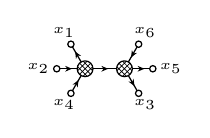
\begin{tikzpicture}[x=0.500cm, y=0.500cm, line width=0.450pt, baseline={([yshift=-0.6ex]0,0)}]
  \draw (-0.500,0.000) -- (-0.860,0.624);
  \fill (-0.753,0.439) -- (-0.731,0.251) -- (-0.695,0.337) -- (-0.602,0.326) -- cycle;
  \draw (0.500,0.000) -- (0.860,-0.624);
  \fill (0.753,-0.439) -- (0.731,-0.251) -- (0.695,-0.337) -- (0.602,-0.326) -- cycle;
  \draw (0.500,0.000) -- (1.220,0.000);
  \fill (1.007,0.000) -- (0.833,0.074) -- (0.890,0.000) -- (0.833,-0.074) -- cycle;
  \draw (-1.220,0.000) -- (-0.500,0.000);
  \fill (-0.833,0.000) -- (-1.007,0.074) -- (-0.950,0.000) -- (-1.007,-0.074) -- cycle;
  \draw (-0.860,-0.624) -- (-0.500,0.000);
  \fill (-0.667,-0.288) -- (-0.818,-0.402) -- (-0.725,-0.390) -- (-0.689,-0.476) -- cycle;
  \draw (0.860,0.624) -- (0.500,0.000);
  \fill (0.667,0.288) -- (0.818,0.402) -- (0.725,0.390) -- (0.689,0.476) -- cycle;
  \draw (-0.500,0.000) -- (0.500,0.000);
  \fill (0.087,0.000) -- (-0.087,0.074) -- (-0.030,0.000) -- (-0.087,-0.074) -- cycle;
  \fill[white] (-0.500,0.000) circle (0.200);
  \draw[line width=0.248pt] (-0.693,-0.052) -- (-0.448,0.193) (-0.641,-0.141) -- (-0.359,0.141) (-0.552,-0.193) -- (-0.307,0.052) (-0.693,0.052) -- (-0.448,-0.193) (-0.641,0.141) -- (-0.359,-0.141) (-0.552,0.193) -- (-0.307,-0.052);
  \draw (-0.500,0.000) circle (0.200);
  \fill[white] (0.500,0.000) circle (0.200);
  \draw[line width=0.248pt] (0.307,-0.052) -- (0.552,0.193) (0.359,-0.141) -- (0.641,0.141) (0.448,-0.193) -- (0.693,0.052) (0.307,0.052) -- (0.552,-0.193) (0.359,0.141) -- (0.641,-0.141) (0.448,0.193) -- (0.693,-0.052);
  \draw (0.500,0.000) circle (0.200);
  \draw[fill=white] (-0.860,0.624) circle (0.080);
  \draw[fill=white] (-1.220,0.000) circle (0.080);
  \draw[fill=white] (0.860,-0.624) circle (0.080);
  \draw[fill=white] (-0.860,-0.624) circle (0.080);
  \draw[fill=white] (1.220,0.000) circle (0.080);
  \draw[fill=white] (0.860,0.624) circle (0.080);
  \node[font=\tiny, inner sep=0pt, anchor=300] at (-0.945,0.771) {$x_{1}$};
  \node[font=\tiny, inner sep=0pt, anchor=0] at (-1.390,0.000) {$x_{2}$};
  \node[font=\tiny, inner sep=0pt, anchor=120] at (0.945,-0.771) {$x_{3}$};
  \node[font=\tiny, inner sep=0pt, anchor=60] at (-0.945,-0.771) {$x_{4}$};
  \node[font=\tiny, inner sep=0pt, anchor=180] at (1.390,0.000) {$x_{5}$};
  \node[font=\tiny, inner sep=0pt, anchor=240] at (0.945,0.771) {$x_{6}$};
\end{tikzpicture}}
\diagramgap
\mbox{$\displaystyle -\,$\,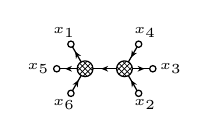
\begin{tikzpicture}[x=0.500cm, y=0.500cm, line width=0.450pt, baseline={([yshift=-0.6ex]0,0)}]
  \draw (-0.500,0.000) -- (-0.860,0.624);
  \fill (-0.753,0.439) -- (-0.731,0.251) -- (-0.695,0.337) -- (-0.602,0.326) -- cycle;
  \draw (0.500,0.000) -- (1.220,0.000);
  \fill (1.007,0.000) -- (0.833,0.074) -- (0.890,0.000) -- (0.833,-0.074) -- cycle;
  \draw (-0.500,0.000) -- (-1.220,0.000);
  \fill (-1.007,0.000) -- (-0.833,-0.074) -- (-0.890,0.000) -- (-0.833,0.074) -- cycle;
  \draw (0.860,-0.624) -- (0.500,0.000);
  \fill (0.667,-0.288) -- (0.689,-0.476) -- (0.725,-0.390) -- (0.818,-0.402) -- cycle;
  \draw (0.860,0.624) -- (0.500,0.000);
  \fill (0.667,0.288) -- (0.818,0.402) -- (0.725,0.390) -- (0.689,0.476) -- cycle;
  \draw (-0.860,-0.624) -- (-0.500,0.000);
  \fill (-0.667,-0.288) -- (-0.818,-0.402) -- (-0.725,-0.390) -- (-0.689,-0.476) -- cycle;
  \draw (0.500,0.000) -- (-0.500,0.000);
  \fill (-0.087,0.000) -- (0.087,-0.074) -- (0.030,0.000) -- (0.087,0.074) -- cycle;
  \fill[white] (-0.500,0.000) circle (0.200);
  \draw[line width=0.248pt] (-0.693,-0.052) -- (-0.448,0.193) (-0.641,-0.141) -- (-0.359,0.141) (-0.552,-0.193) -- (-0.307,0.052) (-0.693,0.052) -- (-0.448,-0.193) (-0.641,0.141) -- (-0.359,-0.141) (-0.552,0.193) -- (-0.307,-0.052);
  \draw (-0.500,0.000) circle (0.200);
  \fill[white] (0.500,0.000) circle (0.200);
  \draw[line width=0.248pt] (0.307,-0.052) -- (0.552,0.193) (0.359,-0.141) -- (0.641,0.141) (0.448,-0.193) -- (0.693,0.052) (0.307,0.052) -- (0.552,-0.193) (0.359,0.141) -- (0.641,-0.141) (0.448,0.193) -- (0.693,-0.052);
  \draw (0.500,0.000) circle (0.200);
  \draw[fill=white] (-0.860,0.624) circle (0.080);
  \draw[fill=white] (0.860,-0.624) circle (0.080);
  \draw[fill=white] (1.220,0.000) circle (0.080);
  \draw[fill=white] (0.860,0.624) circle (0.080);
  \draw[fill=white] (-1.220,0.000) circle (0.080);
  \draw[fill=white] (-0.860,-0.624) circle (0.080);
  \node[font=\tiny, inner sep=0pt, anchor=300] at (-0.945,0.771) {$x_{1}$};
  \node[font=\tiny, inner sep=0pt, anchor=120] at (0.945,-0.771) {$x_{2}$};
  \node[font=\tiny, inner sep=0pt, anchor=180] at (1.390,0.000) {$x_{3}$};
  \node[font=\tiny, inner sep=0pt, anchor=240] at (0.945,0.771) {$x_{4}$};
  \node[font=\tiny, inner sep=0pt, anchor=0] at (-1.390,0.000) {$x_{5}$};
  \node[font=\tiny, inner sep=0pt, anchor=60] at (-0.945,-0.771) {$x_{6}$};
\end{tikzpicture}}
\diagramgap
\mbox{$\displaystyle +\,$\,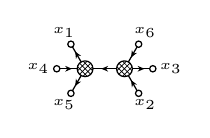
\begin{tikzpicture}[x=0.500cm, y=0.500cm, line width=0.450pt, baseline={([yshift=-0.6ex]0,0)}]
  \draw (-0.500,0.000) -- (-0.860,0.624);
  \fill (-0.753,0.439) -- (-0.731,0.251) -- (-0.695,0.337) -- (-0.602,0.326) -- cycle;
  \draw (0.500,0.000) -- (1.220,0.000);
  \fill (1.007,0.000) -- (0.833,0.074) -- (0.890,0.000) -- (0.833,-0.074) -- cycle;
  \draw (-0.500,0.000) -- (-0.860,-0.624);
  \fill (-0.753,-0.439) -- (-0.602,-0.326) -- (-0.695,-0.337) -- (-0.731,-0.251) -- cycle;
  \draw (0.860,-0.624) -- (0.500,0.000);
  \fill (0.667,-0.288) -- (0.689,-0.476) -- (0.725,-0.390) -- (0.818,-0.402) -- cycle;
  \draw (-1.220,0.000) -- (-0.500,0.000);
  \fill (-0.833,0.000) -- (-1.007,0.074) -- (-0.950,0.000) -- (-1.007,-0.074) -- cycle;
  \draw (0.860,0.624) -- (0.500,0.000);
  \fill (0.667,0.288) -- (0.818,0.402) -- (0.725,0.390) -- (0.689,0.476) -- cycle;
  \draw (0.500,0.000) -- (-0.500,0.000);
  \fill (-0.087,0.000) -- (0.087,-0.074) -- (0.030,0.000) -- (0.087,0.074) -- cycle;
  \fill[white] (-0.500,0.000) circle (0.200);
  \draw[line width=0.248pt] (-0.693,-0.052) -- (-0.448,0.193) (-0.641,-0.141) -- (-0.359,0.141) (-0.552,-0.193) -- (-0.307,0.052) (-0.693,0.052) -- (-0.448,-0.193) (-0.641,0.141) -- (-0.359,-0.141) (-0.552,0.193) -- (-0.307,-0.052);
  \draw (-0.500,0.000) circle (0.200);
  \fill[white] (0.500,0.000) circle (0.200);
  \draw[line width=0.248pt] (0.307,-0.052) -- (0.552,0.193) (0.359,-0.141) -- (0.641,0.141) (0.448,-0.193) -- (0.693,0.052) (0.307,0.052) -- (0.552,-0.193) (0.359,0.141) -- (0.641,-0.141) (0.448,0.193) -- (0.693,-0.052);
  \draw (0.500,0.000) circle (0.200);
  \draw[fill=white] (-0.860,0.624) circle (0.080);
  \draw[fill=white] (0.860,-0.624) circle (0.080);
  \draw[fill=white] (1.220,0.000) circle (0.080);
  \draw[fill=white] (-1.220,0.000) circle (0.080);
  \draw[fill=white] (-0.860,-0.624) circle (0.080);
  \draw[fill=white] (0.860,0.624) circle (0.080);
  \node[font=\tiny, inner sep=0pt, anchor=300] at (-0.945,0.771) {$x_{1}$};
  \node[font=\tiny, inner sep=0pt, anchor=120] at (0.945,-0.771) {$x_{2}$};
  \node[font=\tiny, inner sep=0pt, anchor=180] at (1.390,0.000) {$x_{3}$};
  \node[font=\tiny, inner sep=0pt, anchor=0] at (-1.390,0.000) {$x_{4}$};
  \node[font=\tiny, inner sep=0pt, anchor=60] at (-0.945,-0.771) {$x_{5}$};
  \node[font=\tiny, inner sep=0pt, anchor=240] at (0.945,0.771) {$x_{6}$};
\end{tikzpicture}}
\diagramgap
\mbox{$\displaystyle -\,$\,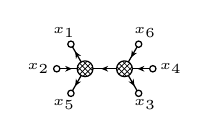
\begin{tikzpicture}[x=0.500cm, y=0.500cm, line width=0.450pt, baseline={([yshift=-0.6ex]0,0)}]
  \draw (-0.500,0.000) -- (-0.860,0.624);
  \fill (-0.753,0.439) -- (-0.731,0.251) -- (-0.695,0.337) -- (-0.602,0.326) -- cycle;
  \draw (0.500,0.000) -- (0.860,-0.624);
  \fill (0.753,-0.439) -- (0.731,-0.251) -- (0.695,-0.337) -- (0.602,-0.326) -- cycle;
  \draw (-0.500,0.000) -- (-0.860,-0.624);
  \fill (-0.753,-0.439) -- (-0.602,-0.326) -- (-0.695,-0.337) -- (-0.731,-0.251) -- cycle;
  \draw (-1.220,0.000) -- (-0.500,0.000);
  \fill (-0.833,0.000) -- (-1.007,0.074) -- (-0.950,0.000) -- (-1.007,-0.074) -- cycle;
  \draw (1.220,0.000) -- (0.500,0.000);
  \fill (0.833,0.000) -- (1.007,-0.074) -- (0.950,0.000) -- (1.007,0.074) -- cycle;
  \draw (0.860,0.624) -- (0.500,0.000);
  \fill (0.667,0.288) -- (0.818,0.402) -- (0.725,0.390) -- (0.689,0.476) -- cycle;
  \draw (0.500,0.000) -- (-0.500,0.000);
  \fill (-0.087,0.000) -- (0.087,-0.074) -- (0.030,0.000) -- (0.087,0.074) -- cycle;
  \fill[white] (-0.500,0.000) circle (0.200);
  \draw[line width=0.248pt] (-0.693,-0.052) -- (-0.448,0.193) (-0.641,-0.141) -- (-0.359,0.141) (-0.552,-0.193) -- (-0.307,0.052) (-0.693,0.052) -- (-0.448,-0.193) (-0.641,0.141) -- (-0.359,-0.141) (-0.552,0.193) -- (-0.307,-0.052);
  \draw (-0.500,0.000) circle (0.200);
  \fill[white] (0.500,0.000) circle (0.200);
  \draw[line width=0.248pt] (0.307,-0.052) -- (0.552,0.193) (0.359,-0.141) -- (0.641,0.141) (0.448,-0.193) -- (0.693,0.052) (0.307,0.052) -- (0.552,-0.193) (0.359,0.141) -- (0.641,-0.141) (0.448,0.193) -- (0.693,-0.052);
  \draw (0.500,0.000) circle (0.200);
  \draw[fill=white] (-0.860,0.624) circle (0.080);
  \draw[fill=white] (-1.220,0.000) circle (0.080);
  \draw[fill=white] (0.860,-0.624) circle (0.080);
  \draw[fill=white] (1.220,0.000) circle (0.080);
  \draw[fill=white] (-0.860,-0.624) circle (0.080);
  \draw[fill=white] (0.860,0.624) circle (0.080);
  \node[font=\tiny, inner sep=0pt, anchor=300] at (-0.945,0.771) {$x_{1}$};
  \node[font=\tiny, inner sep=0pt, anchor=0] at (-1.390,0.000) {$x_{2}$};
  \node[font=\tiny, inner sep=0pt, anchor=120] at (0.945,-0.771) {$x_{3}$};
  \node[font=\tiny, inner sep=0pt, anchor=180] at (1.390,0.000) {$x_{4}$};
  \node[font=\tiny, inner sep=0pt, anchor=60] at (-0.945,-0.771) {$x_{5}$};
  \node[font=\tiny, inner sep=0pt, anchor=240] at (0.945,0.771) {$x_{6}$};
\end{tikzpicture}}
\diagramgap
\mbox{$\displaystyle +\,$\,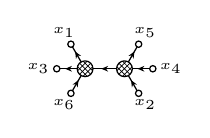
\begin{tikzpicture}[x=0.500cm, y=0.500cm, line width=0.450pt, baseline={([yshift=-0.6ex]0,0)}]
  \draw (-0.500,0.000) -- (-0.860,0.624);
  \fill (-0.753,0.439) -- (-0.731,0.251) -- (-0.695,0.337) -- (-0.602,0.326) -- cycle;
  \draw (-0.500,0.000) -- (-1.220,0.000);
  \fill (-1.007,0.000) -- (-0.833,-0.074) -- (-0.890,0.000) -- (-0.833,0.074) -- cycle;
  \draw (0.500,0.000) -- (0.860,0.624);
  \fill (0.753,0.439) -- (0.602,0.326) -- (0.695,0.337) -- (0.731,0.251) -- cycle;
  \draw (0.860,-0.624) -- (0.500,0.000);
  \fill (0.667,-0.288) -- (0.689,-0.476) -- (0.725,-0.390) -- (0.818,-0.402) -- cycle;
  \draw (1.220,0.000) -- (0.500,0.000);
  \fill (0.833,0.000) -- (1.007,-0.074) -- (0.950,0.000) -- (1.007,0.074) -- cycle;
  \draw (-0.860,-0.624) -- (-0.500,0.000);
  \fill (-0.667,-0.288) -- (-0.818,-0.402) -- (-0.725,-0.390) -- (-0.689,-0.476) -- cycle;
  \draw (0.500,0.000) -- (-0.500,0.000);
  \fill (-0.087,0.000) -- (0.087,-0.074) -- (0.030,0.000) -- (0.087,0.074) -- cycle;
  \fill[white] (-0.500,0.000) circle (0.200);
  \draw[line width=0.248pt] (-0.693,-0.052) -- (-0.448,0.193) (-0.641,-0.141) -- (-0.359,0.141) (-0.552,-0.193) -- (-0.307,0.052) (-0.693,0.052) -- (-0.448,-0.193) (-0.641,0.141) -- (-0.359,-0.141) (-0.552,0.193) -- (-0.307,-0.052);
  \draw (-0.500,0.000) circle (0.200);
  \fill[white] (0.500,0.000) circle (0.200);
  \draw[line width=0.248pt] (0.307,-0.052) -- (0.552,0.193) (0.359,-0.141) -- (0.641,0.141) (0.448,-0.193) -- (0.693,0.052) (0.307,0.052) -- (0.552,-0.193) (0.359,0.141) -- (0.641,-0.141) (0.448,0.193) -- (0.693,-0.052);
  \draw (0.500,0.000) circle (0.200);
  \draw[fill=white] (-0.860,0.624) circle (0.080);
  \draw[fill=white] (0.860,-0.624) circle (0.080);
  \draw[fill=white] (-1.220,0.000) circle (0.080);
  \draw[fill=white] (1.220,0.000) circle (0.080);
  \draw[fill=white] (0.860,0.624) circle (0.080);
  \draw[fill=white] (-0.860,-0.624) circle (0.080);
  \node[font=\tiny, inner sep=0pt, anchor=300] at (-0.945,0.771) {$x_{1}$};
  \node[font=\tiny, inner sep=0pt, anchor=120] at (0.945,-0.771) {$x_{2}$};
  \node[font=\tiny, inner sep=0pt, anchor=0] at (-1.390,0.000) {$x_{3}$};
  \node[font=\tiny, inner sep=0pt, anchor=180] at (1.390,0.000) {$x_{4}$};
  \node[font=\tiny, inner sep=0pt, anchor=240] at (0.945,0.771) {$x_{5}$};
  \node[font=\tiny, inner sep=0pt, anchor=60] at (-0.945,-0.771) {$x_{6}$};
\end{tikzpicture}}
\diagramgap
\mbox{$\displaystyle -\,$\,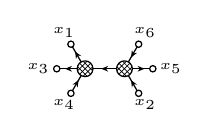
\begin{tikzpicture}[x=0.500cm, y=0.500cm, line width=0.450pt, baseline={([yshift=-0.6ex]0,0)}]
  \draw (-0.500,0.000) -- (-0.860,0.624);
  \fill (-0.753,0.439) -- (-0.731,0.251) -- (-0.695,0.337) -- (-0.602,0.326) -- cycle;
  \draw (-0.500,0.000) -- (-1.220,0.000);
  \fill (-1.007,0.000) -- (-0.833,-0.074) -- (-0.890,0.000) -- (-0.833,0.074) -- cycle;
  \draw (0.500,0.000) -- (1.220,0.000);
  \fill (1.007,0.000) -- (0.833,0.074) -- (0.890,0.000) -- (0.833,-0.074) -- cycle;
  \draw (0.860,-0.624) -- (0.500,0.000);
  \fill (0.667,-0.288) -- (0.689,-0.476) -- (0.725,-0.390) -- (0.818,-0.402) -- cycle;
  \draw (-0.860,-0.624) -- (-0.500,0.000);
  \fill (-0.667,-0.288) -- (-0.818,-0.402) -- (-0.725,-0.390) -- (-0.689,-0.476) -- cycle;
  \draw (0.860,0.624) -- (0.500,0.000);
  \fill (0.667,0.288) -- (0.818,0.402) -- (0.725,0.390) -- (0.689,0.476) -- cycle;
  \draw (0.500,0.000) -- (-0.500,0.000);
  \fill (-0.087,0.000) -- (0.087,-0.074) -- (0.030,0.000) -- (0.087,0.074) -- cycle;
  \fill[white] (-0.500,0.000) circle (0.200);
  \draw[line width=0.248pt] (-0.693,-0.052) -- (-0.448,0.193) (-0.641,-0.141) -- (-0.359,0.141) (-0.552,-0.193) -- (-0.307,0.052) (-0.693,0.052) -- (-0.448,-0.193) (-0.641,0.141) -- (-0.359,-0.141) (-0.552,0.193) -- (-0.307,-0.052);
  \draw (-0.500,0.000) circle (0.200);
  \fill[white] (0.500,0.000) circle (0.200);
  \draw[line width=0.248pt] (0.307,-0.052) -- (0.552,0.193) (0.359,-0.141) -- (0.641,0.141) (0.448,-0.193) -- (0.693,0.052) (0.307,0.052) -- (0.552,-0.193) (0.359,0.141) -- (0.641,-0.141) (0.448,0.193) -- (0.693,-0.052);
  \draw (0.500,0.000) circle (0.200);
  \draw[fill=white] (-0.860,0.624) circle (0.080);
  \draw[fill=white] (0.860,-0.624) circle (0.080);
  \draw[fill=white] (-1.220,0.000) circle (0.080);
  \draw[fill=white] (-0.860,-0.624) circle (0.080);
  \draw[fill=white] (1.220,0.000) circle (0.080);
  \draw[fill=white] (0.860,0.624) circle (0.080);
  \node[font=\tiny, inner sep=0pt, anchor=300] at (-0.945,0.771) {$x_{1}$};
  \node[font=\tiny, inner sep=0pt, anchor=120] at (0.945,-0.771) {$x_{2}$};
  \node[font=\tiny, inner sep=0pt, anchor=0] at (-1.390,0.000) {$x_{3}$};
  \node[font=\tiny, inner sep=0pt, anchor=60] at (-0.945,-0.771) {$x_{4}$};
  \node[font=\tiny, inner sep=0pt, anchor=180] at (1.390,0.000) {$x_{5}$};
  \node[font=\tiny, inner sep=0pt, anchor=240] at (0.945,0.771) {$x_{6}$};
\end{tikzpicture}}
\diagramgap
\mbox{$\displaystyle +\,$\,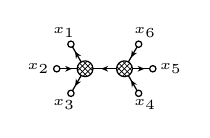
\begin{tikzpicture}[x=0.500cm, y=0.500cm, line width=0.450pt, baseline={([yshift=-0.6ex]0,0)}]
  \draw (-0.500,0.000) -- (-0.860,0.624);
  \fill (-0.753,0.439) -- (-0.731,0.251) -- (-0.695,0.337) -- (-0.602,0.326) -- cycle;
  \draw (-0.500,0.000) -- (-0.860,-0.624);
  \fill (-0.753,-0.439) -- (-0.602,-0.326) -- (-0.695,-0.337) -- (-0.731,-0.251) -- cycle;
  \draw (0.500,0.000) -- (1.220,0.000);
  \fill (1.007,0.000) -- (0.833,0.074) -- (0.890,0.000) -- (0.833,-0.074) -- cycle;
  \draw (-1.220,0.000) -- (-0.500,0.000);
  \fill (-0.833,0.000) -- (-1.007,0.074) -- (-0.950,0.000) -- (-1.007,-0.074) -- cycle;
  \draw (0.860,-0.624) -- (0.500,0.000);
  \fill (0.667,-0.288) -- (0.689,-0.476) -- (0.725,-0.390) -- (0.818,-0.402) -- cycle;
  \draw (0.860,0.624) -- (0.500,0.000);
  \fill (0.667,0.288) -- (0.818,0.402) -- (0.725,0.390) -- (0.689,0.476) -- cycle;
  \draw (0.500,0.000) -- (-0.500,0.000);
  \fill (-0.087,0.000) -- (0.087,-0.074) -- (0.030,0.000) -- (0.087,0.074) -- cycle;
  \fill[white] (-0.500,0.000) circle (0.200);
  \draw[line width=0.248pt] (-0.693,-0.052) -- (-0.448,0.193) (-0.641,-0.141) -- (-0.359,0.141) (-0.552,-0.193) -- (-0.307,0.052) (-0.693,0.052) -- (-0.448,-0.193) (-0.641,0.141) -- (-0.359,-0.141) (-0.552,0.193) -- (-0.307,-0.052);
  \draw (-0.500,0.000) circle (0.200);
  \fill[white] (0.500,0.000) circle (0.200);
  \draw[line width=0.248pt] (0.307,-0.052) -- (0.552,0.193) (0.359,-0.141) -- (0.641,0.141) (0.448,-0.193) -- (0.693,0.052) (0.307,0.052) -- (0.552,-0.193) (0.359,0.141) -- (0.641,-0.141) (0.448,0.193) -- (0.693,-0.052);
  \draw (0.500,0.000) circle (0.200);
  \draw[fill=white] (-0.860,0.624) circle (0.080);
  \draw[fill=white] (-1.220,0.000) circle (0.080);
  \draw[fill=white] (-0.860,-0.624) circle (0.080);
  \draw[fill=white] (0.860,-0.624) circle (0.080);
  \draw[fill=white] (1.220,0.000) circle (0.080);
  \draw[fill=white] (0.860,0.624) circle (0.080);
  \node[font=\tiny, inner sep=0pt, anchor=300] at (-0.945,0.771) {$x_{1}$};
  \node[font=\tiny, inner sep=0pt, anchor=0] at (-1.390,0.000) {$x_{2}$};
  \node[font=\tiny, inner sep=0pt, anchor=60] at (-0.945,-0.771) {$x_{3}$};
  \node[font=\tiny, inner sep=0pt, anchor=120] at (0.945,-0.771) {$x_{4}$};
  \node[font=\tiny, inner sep=0pt, anchor=180] at (1.390,0.000) {$x_{5}$};
  \node[font=\tiny, inner sep=0pt, anchor=240] at (0.945,0.771) {$x_{6}$};
\end{tikzpicture}}
